\documentclass{beamer}
\usepackage[utf8]{inputenc}
\usepackage{graphicx}
\usetheme{Warsaw}
\usecolortheme{seahorse}

\title{Cancer Analysis Workflow Sprint Review}
\institute{SciLifeLab}
\date{13th Oct. 2016 }
\begin{document}
\frame{\titlepage}
			  
\begin{frame}
\frametitle{Cancer Analysis Workflow Sprint Review}
\begin{itemize}
	\item Which parts are ready so far?
	\item Things waiting to be completed
	\item Yet to come
\end{itemize}
\end{frame}

\begin{frame}
\frametitle{Where Are We Now?}
Expected to present DREAM challenge comparisons by now - still a dream, no variant call comparisons yet.
	\begin{block}{\#include \textless usual\_excuse.h\textgreater}
	Besides resource (CPU/disk) shortage the software have to be re-designed in a way that it can use preprocessed data
	and we do not have to align/realign/recalibrate from scratch.
	\end{block}
	\begin{itemize}
		\item with re-design and adding new features we still gained time
		\item comparing VCFs is not that straightforward
		\item on a side-note: realignment will be gone eventually
	\end{itemize}
\end{frame}

\begin{frame}
\frametitle{Where Are We Now?}
	\begin{block}{To be ready for benchmarking}
		NGI Production is delivering realigned BAMs with recalibration table for a while

		To reanalyse old data we have to have a way to start from a different entry point

		\begin{itemize}
			\item ... from scratch FASTQ
			\item ... from some other part of the preprocessing pipeline
			\item ... running only particular variant callers or statistical software
		\end{itemize}
		Maxime is to give details
	\end{block}
\end{frame}

\begin{frame}
\frametitle{Cancer Analysis Workflow Sprint Review}
\begin{itemize}
	\item Which parts are ready so far?
		\begin{itemize}
			\item Preprocessing
			\item Normal / Tumour / Relapse steps, read groups
			\item Strelka, MuTect1 as default callers
			\item MuTect2 and VarDict if you have enough memory
			\item ASCAT, Manta integrated
			\item Germline variants HaplotypeCaller
			\item public GitHub repo - in the awesome flow list
			\item I/O CPU time benchmarks
			\item Malin already used the flow for real data
		\end{itemize}
	\item Things waiting to be completed
		\begin{itemize}
			\item merging results
			\item benchmarking
		\end{itemize}
	\item Yet to come
		\begin{itemize}
			\item Annotation (prototype is ready)
			\item Visualization
			\item Data mining / AI / SVM to eliminate false positives
		\end{itemize}
\end{itemize}
\end{frame}

\begin{frame}
\frametitle{Germline variants}
	\begin{block}{Preprocessing is the same as for GATK-BP}
	Just like NGI WGS pipeline now in production

	Using more up-to-date versions of tools (bugfixes, new features)

	Sebastian's first nextflow contribution
	\end{block}
	\begin{itemize}
		\item GATK HaplotypeCaller for germline variants
		\item We have to compare the two pipelines for validation
		\item Do we have something already in place for germline prioritization/annotation?
	\end{itemize}
\end{frame}

\begin{frame}
\frametitle{UPPMAX/SNIC resources used}
	\begin{block}{UPPMAX clusters targeted}
		\begin{itemize}
			\item most of the testing on milou
			\item test runs on irma
			\item SNIC asked us to run pilot studies on bianca
			\item Still, data to be stored on PDC
		\end{itemize}
	\end{block}
	Bianca is a new cluster for research projects, with large storage capacity, many CPUs and modern hardware.
	Designed for projects with sensitive data and scheduled for Q1 2017. In Nov-Dec we could use it for cancer pilot
	projects, almost exclusively. 
\end{frame}

\begin{frame}
\frametitle{Data storage}
	\begin{block}{Main concern: storage}
	NGI is storing data for 3 months after closing a project. Neither irma nor bianca is suitable for long-term data
	storage. Have to find solution (either PDC, or local storage or both) for/by the users. 
	\end{block}
	In practice: 
	\begin{itemize}
		\item 250 GB input FASTQ generates 1700 GB temporary data (7x storage increase)
		\item only the result of preprocessing (realigned and recalibrated BAM) that is interesting
		\item up/downloading to PDC takes time (hours)
		\item recalibration takes even more time (but the storage on PDC is smaller)
	\end{itemize}
\end{frame}

\begin{frame}
\frametitle{Data storage}
	\begin{itemize}
		\item The realigned data is about 290 GB, it takes 180h single core CPU time ($\sim$12h on an irma node with 16 cores)
		to get recalibrated BAMs.
		\item Other option is to store the recalibrated BAMs, that is about 500 GB -- twice the input data.
		\item in this case you do not	have to store initial FASTQs, and files are immediately suitable for further analysis.
		Download from PDC is 3 hours max.
	\end{itemize}
\end{frame}

\begin{frame}
\frametitle{Storage/CPU benchmarks}
\center { 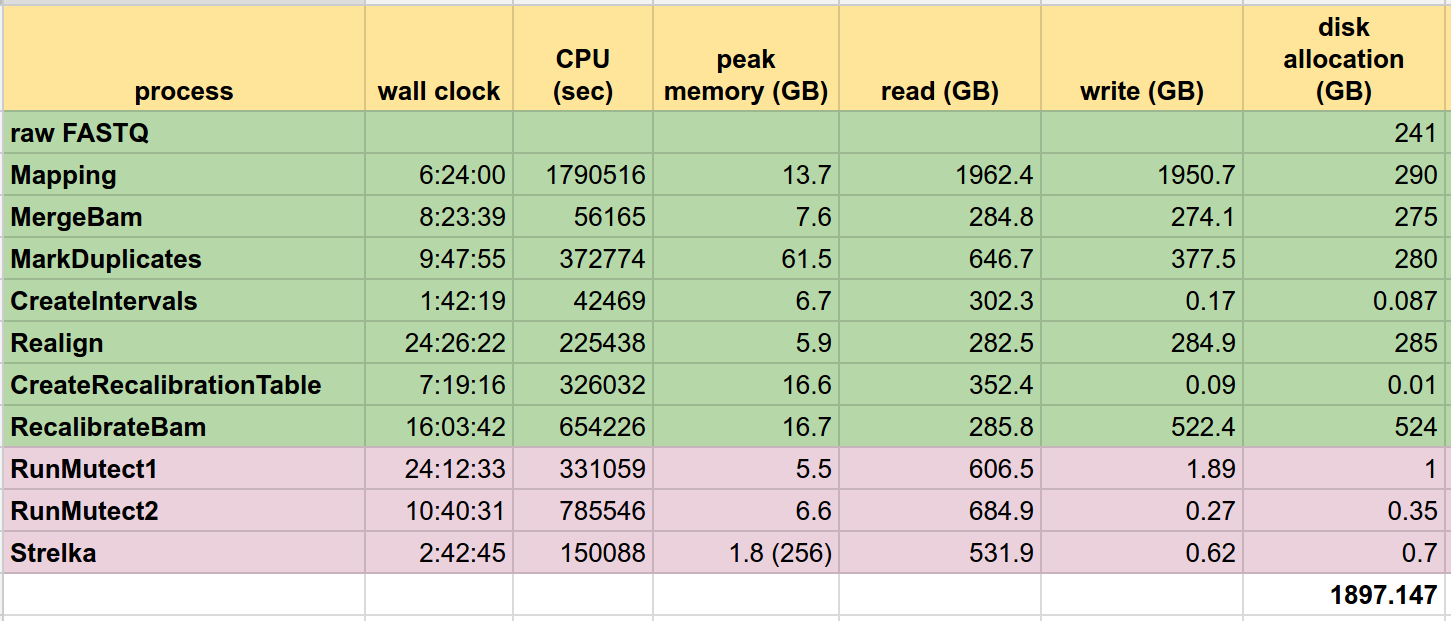
\includegraphics[width=1\linewidth]{Irma_timings.png} }
\end{frame}

\begin{frame}
\frametitle{Other bits and pieces}
\begin{itemize}
	\item GitHub public repo lesson: if you moving to public, think twice, and make it public from the beginning
	\item New name? Seems CAPS, SNAP is on the lead after four of us voting
	\item http://doodle.com/poll/k9hxggtysbdnfdg4 
\end{itemize}
\end{frame}

\begin{frame}
\frametitle{TODO / next sprint}
	\begin{itemize}
		\item Malin is going to give a presentation about ASCAT this afternoon 13:00 in Alpha 3 Black Hole
		\item Merge variant calls from different callers into a singe result file
		\item Go through all the TCGA DREAM challenge benchmarking steps S1, S2, S3
		\item Next meeting at ?
	\end{itemize}
\end{frame}

\begin{frame}
\frametitle{The Alphabetical List}
\begin{itemize}
	\item Jesper Eisfeldt
	\item Sebastian DiLorenzo
	\item Maxime Garcia 
	\item Szilveszter Juhos 
	\item Max Käller
	\item Malin Larsson
	\item Björn Nystedt 
	\item Pall Olason
	\item Pelin Sahlen
	\item Teresita Díaz De Ståhl
\end{itemize}
\end{frame}

\end{document}
